\frame{
\frametitle{Redes Neurais}
\begin{block}{}
\begin{figure}[H]
\centering
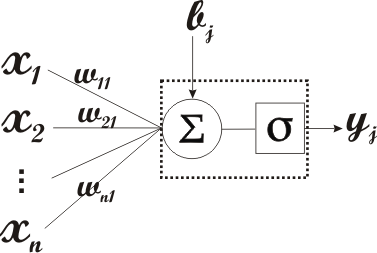
\includegraphics[width=10cm]{figuras/rede_neural_neuronio}
\caption{Modelo matemático de um neurônio.}
\end{figure}
\end{block}
}

\frame{
\frametitle{Redes Neurais}
\begin{block}{}
\begin{figure}[H]
\centering
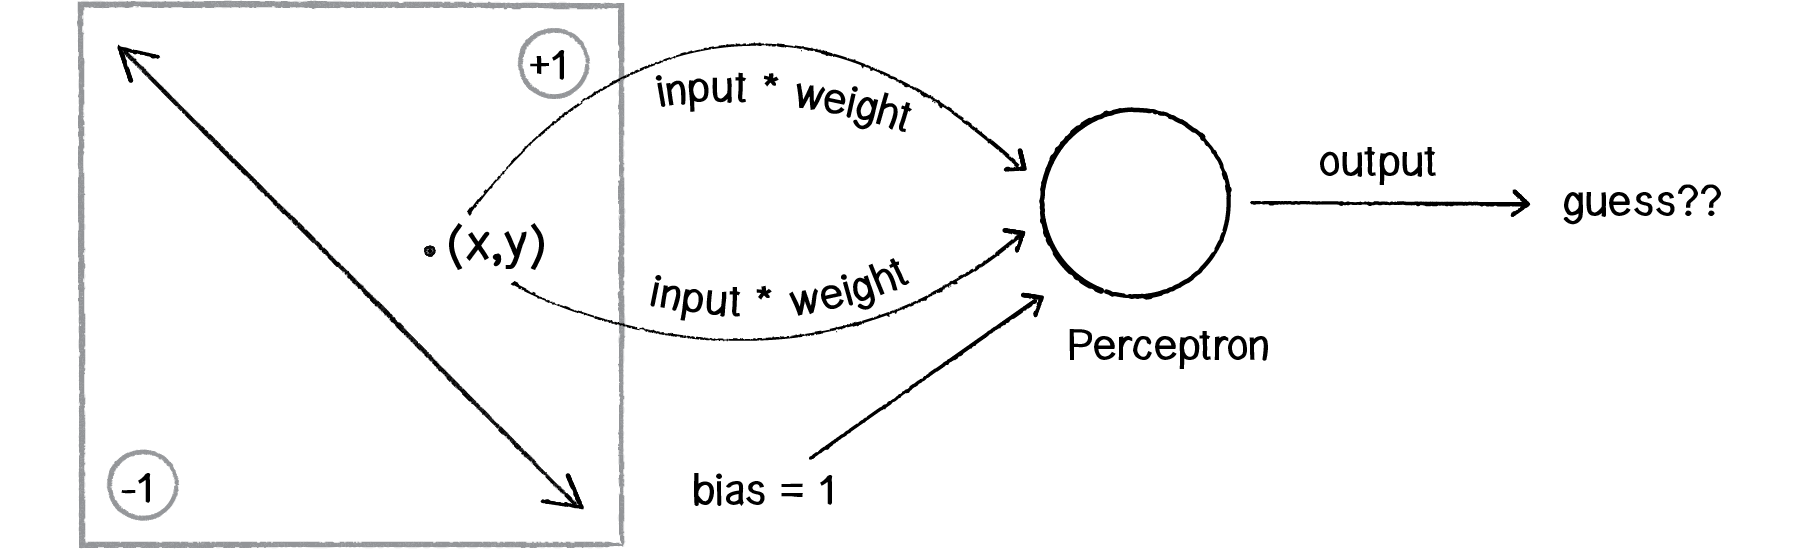
\includegraphics[width=10cm]{figuras/rede_neural_simple_problem}
\caption{\textit{Perceptron} para decidir região de um ponto no plano.}
\end{figure}
\end{block}
}

\frame{
\frametitle{Redes Neurais}
\begin{block}{}
\begin{figure}[H]
\centering
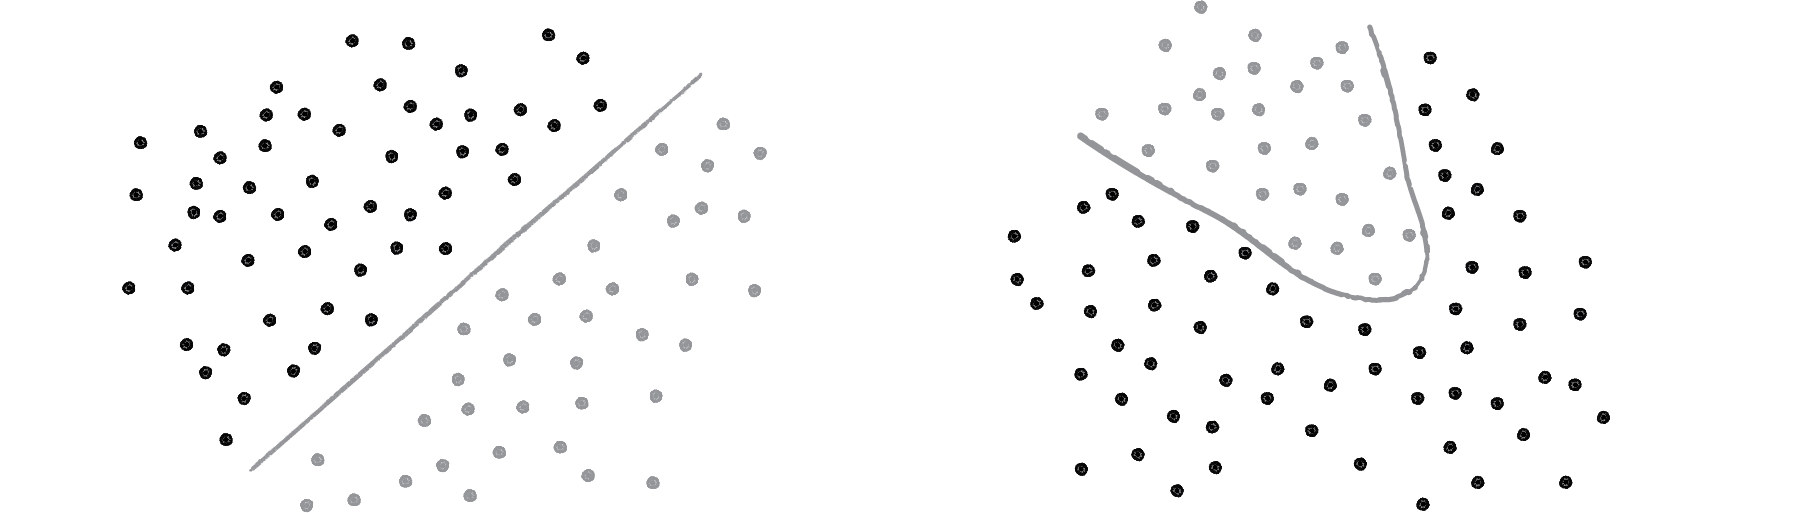
\includegraphics[width=10cm]{figuras/rede_neural_linear_probl}
\caption{Problemas linearmente separáveis vs. não linearmente separáveis.}
\end{figure}
\end{block}
}

\frame{
\frametitle{Redes Neurais}
\begin{block}{}
\begin{figure}[H]
\centering
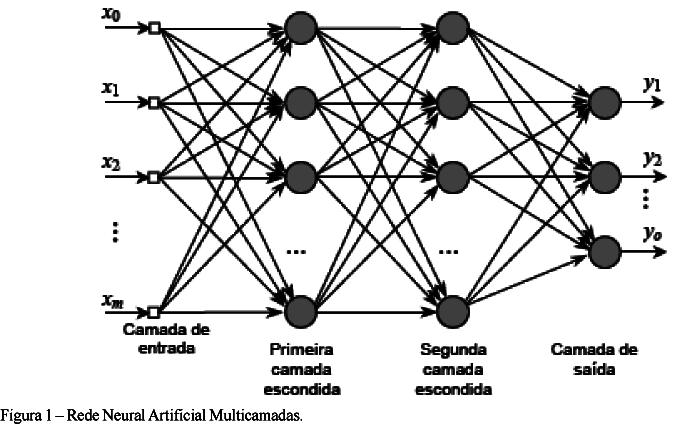
\includegraphics[width=8cm]{figuras/rede_neural_topologia}
\caption{Topologia de camadas.}
\end{figure}
\end{block}
}
